\documentclass{article}

\usepackage[utf8]{inputenc}
\usepackage{titlesec}
\PassOptionsToPackage{hyphens}{url}\usepackage{hyperref}
\usepackage{listings}
\usepackage{graphicx}
\usepackage{float}
\usepackage{xcolor}
\usepackage{csquotes}
\usepackage{lettrine}


\title{ Final Report of Semantic Web about \\ \Huge \textbf{Food}}
\author{Aspir Ahmet \\ Tobias Dick \\ Daniel Egger \\Stefan Kaufmann}
\date{14.02.2019}


\begin{document}
\thispagestyle{empty}
\clearpage
\maketitle
\thispagestyle{empty}
\thispagestyle{empty}
\newpage
\clearpage
\tableofcontents 
\thispagestyle{empty}
\newpage
\pagebreak
\pagenumbering{arabic}
	
\section{Introduction}
This knowledge-graph recipe application serves as an online recipe-look-up service. Either by entering certain ingredients, selecting health labels and diet labels or combing both of the previously mentioned, the request will yield according results. A web-overlay ensures the interaction with regular users. 
\subsection{Use Case}
This application can be used by everyone who is looking for new and refreshing recipes. However it is especially useful for people who are doing a diet or for people whose nutrition is restricted by certain allergies. \\ \\
People who just want to try out new recipes with certain ingredients can easily add those ingredients to the search. After the search process they will receive only recipes containing all the given ingredients as a result.

\subsection{Data Sources}
On the search for useful data sources for a lot of different recipes we came across an API called Edamam. Edamam organizes the worlds food knowledge in one database and is free to use. The database contains over 1.7 million different recipes which can easily be crawled by a simple java program. This way it provides us with tons of different recipes and a lot of information for each recipe. This information contains obvious properties like the recipe name, cook time and ingredients, but it also contains exact health and diet labels for every recipe. Since the given information is so rich, Edamam has been our main data source since the beginning of the project. \\ \\
Anther data source we have been using for a large part of the semester is a small online data set. This data set is free to use and contains about 520 different recipes. However the information provided for each recipe is very minor. This finally led to the exclusion of the data set from our data sources. The main reason for the exclusion is, that the recipes from the small data set would violate the validation through our SHACL shapes. This however will be explained in more detail in a later section.\\ \\
In both cases the data was provided in JSON format, which made the parsing and further storing of the recipes pretty easy.

\subsection{Ontology}
Our first idea was to use schema.org because of its popularity. We were able to find a schema.org class that fitted our intentions perfectly. The main class is $<$\url{https://schema.org/Recipe}$>$ which contains its own recipe properties as well as properties of  $<$\url{https://schema.org/HowTo}$>$, $<$\url{https://schema.org/CreativeWork}$>$ and $<$\url{https://schema.org/Thing}$>$. Given these properties we were able to map most of the recipe attributes, which we use in our application. However not all of them could be mapped to a fitting property. Therefore an extension of the ontology was needed. \\ \\
The first extension made was targeted at the poperty recipeIngredient. In the recipe class from schema.org the recipeIngredient property only consists of a simple text. This however is not sufficient for our purpose since our application requires us to save recipe ingredients as seen in Figure \ref{fig:recipeIngredient}. Unfortunately we were not able to find an existing ontology which would provide this exact structure. Therefore we extended the base vocabulary from schema.org with our own extension for recipeIngredient. 
\begin{figure}[H]
  \centering
  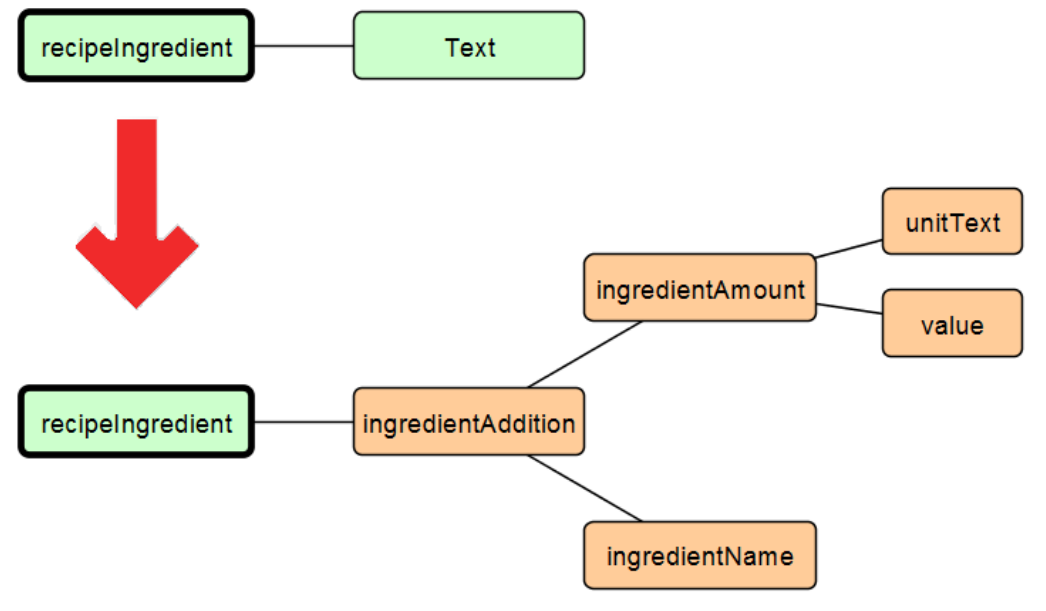
\includegraphics[width=12cm]{pictures/recipeIngredient.png}
  \caption{recipeIngredient Extension}
  \label{fig:recipeIngredient}
\end{figure}
\noindent
\\ \\
The recipe class of schema.org also does not contain a property for a recipes cuisine. For our application or respectively our crawling process this property makes a lot of sense, since we crawl for different recipes dependent on their cuisine. This led to the second extension of our used ontology. In contrast to the first extension we were able to find an existing ontology which contains a cuisine property. This new ontology is an explicit food ontology and can be found at $<$\url{https://www.bbc.co.uk/ontologies/fo}$>$. \\ \\
Given these extensions our final ontology can be seen in Figure \ref{fig:ontology}.    

\begin{figure}[H]
  \centering
  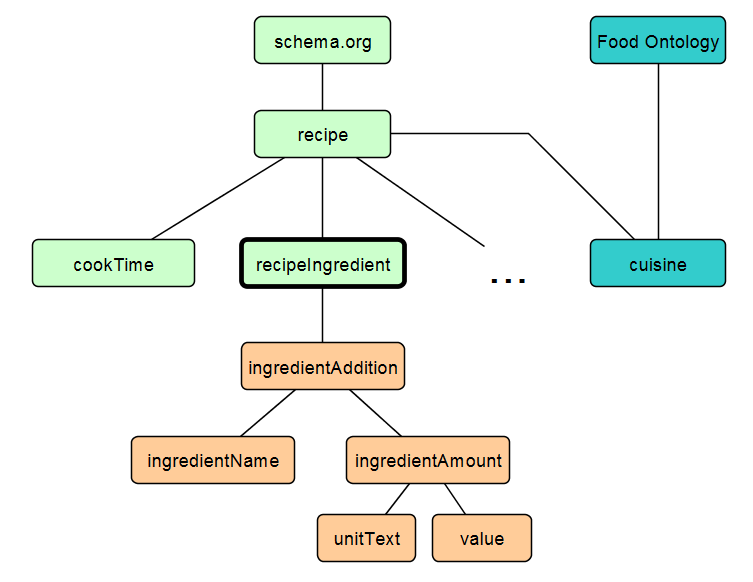
\includegraphics[width=12cm]{pictures/ontology.png}
  \caption{The final Ontology}
  \label{fig:ontology}
\end{figure}
\noindent

\section{Enrichment}
\subsection{Information Extraction - NLP}
As discussed in the previous section all of our recipes come from the Edamam API. However this API provides the recipe ingredients as simple ingredient-lines, which can be seen in Figure \ref{fig:ingredientLines}. But the extension we have made to our ontology regarding recipeIngredient requires us to save every ingredient with a name, an unit text and an amount. Therefore  we have to extract the needed information from this ingredient-lines. This however is not that simple because every line can look different, which makes a common parser useless. 

\begin{figure}[H]
  \centering
  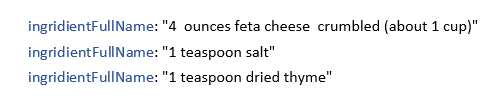
\includegraphics[width=12cm]{pictures/ingredientLines.png}
  \caption{Three Ingredient-Lines}
  \label{fig:ingredientLines}
\end{figure}
\noindent
\\ \\
To achieve a valid parsing we used natural language processing (NLP). NLP is a field of machine learning that seeks to understand human languages and provides specific tools to extract pieces of information, such as NER (named-entity recognition). We have used the Stanford NER tagger on a tokenized version of the corresponding ingredient-line. An example for such a tokenized and tagged ingredient-line is shown in Figure \ref{fig:tokens}. 

\begin{figure}[H]
  \centering
  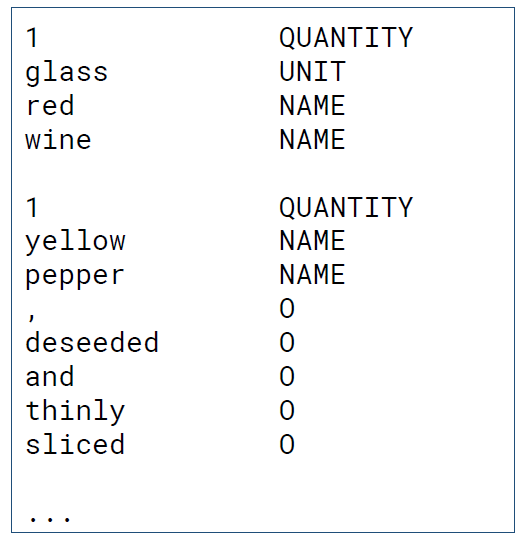
\includegraphics[width=6cm]{pictures/tokens.png}
  \caption{Tokenized Ingredient-Line}
  \label{fig:tokens}
\end{figure}
\noindent
\\ \\
Since we needed to achieve a high accuracy with the named-entity recognition, so that our ingredients would be parsed the right way, we manually created a training model which was specific for our data set. An example of what we achieved with this strategy is shown in Figure \ref{fig:nlp}.

\begin{figure}[H]
  \centering
  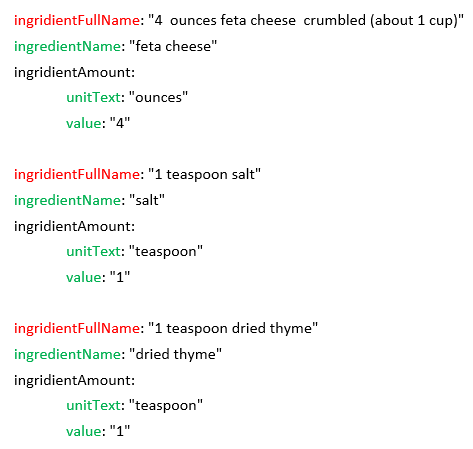
\includegraphics[width=12cm]{pictures/nlp.png}
  \caption{Achived Example Results with NLP}
  \label{fig:nlp}
\end{figure}
\noindent

\subsection{LOD Linking}
\subsubsection{Data Alignment and the Federated Query}
The goal of data alignment is to align our data types with already existing and widely used types. Prime-example for this is Wikidata. Using Wikidatas SPARQL-Endpoint it is possible to find equivalent classes to locally used classes. In this case only schema:Recipe was aligned but it is totally possible to find an alignment for all locally used classes and integrate the Wikidata classes into the ontology in an automated fashion. This requires certain steps such as: Load all yielded Class-Codes from Wikidata to a lookup-table, using a script integrate all loaded Class-Codes into existing ontology via ``Protege''. This was not necessary hence only a demonstrative federated query was included. \\ \\
The used federated query is shown in Figure \ref{fig:fed}:

\begin{figure}[H]
  \centering
  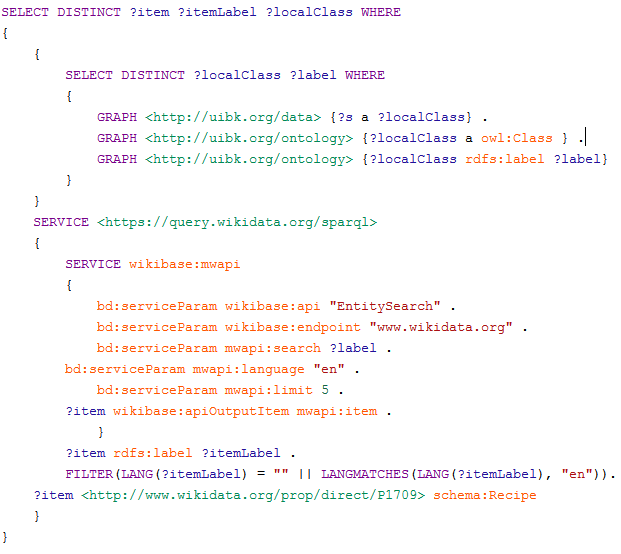
\includegraphics[width=12cm]{pictures/fed_query2.png}
  \caption{Our Federated Query}
  \label{fig:fed}
\end{figure}
\noindent
\\ \\
The first part of the query focuses on getting all locally used classes and their labels '?localClass' '?label'. Once these are known using the keyword 'SERVICE' an external query-service is consulted (Wikidata in this case). On top of the normal usual SPARQL-Query service Wikidata offers a Search-API (MediaWiki SearchAPI) which comes in handy since the labels of the local classes can simply be entered in that API which then returns the according search-results. The part 'SERVICE wikibase:mwapi' returns the Wikidata objects into '?item' which is then further used. The API-Request can be modified by changing the according 'bd:serviceParam'. When finally receiving entries as '?item' from the API a simple query is submitted to find the labels which are then displayed at the local triple store that requested the SERVICE. The last line '?item $<$\url{http://www.wikidata.org/prop/direct/P1709}$>$ schema:Recipe' is to filter to our locally used class schema:Recipe since Wikidata offers a direct equivalence property to 'schema.org' classes. In general the rest of this query could have been avoided, but for reasons mentioned earlier it is useful to leave it in anyway. The result of the query can be seen in Figure \ref{fig:fed_res}:

\begin{figure}[H]
  \centering
  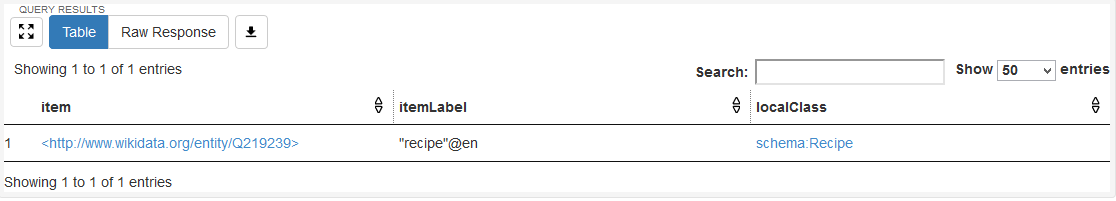
\includegraphics[width=12cm]{pictures/fed_query_result.png}
  \caption{The result of the federated Query}
  \label{fig:fed_res}
\end{figure}
\noindent

\subsubsection{Linking with Entity of Wikidata}
As seen in the previous section we get the corresponding identifier ``Q219239'' from Wikidata as a result from our federated Query. Now we want to link our schema:Recipe with Wikidata (more specific: with the given identifier). To do so we used the program ``Protege'' (Figure \ref{fig:lod}) :

\begin{figure}[H]
  \centering
  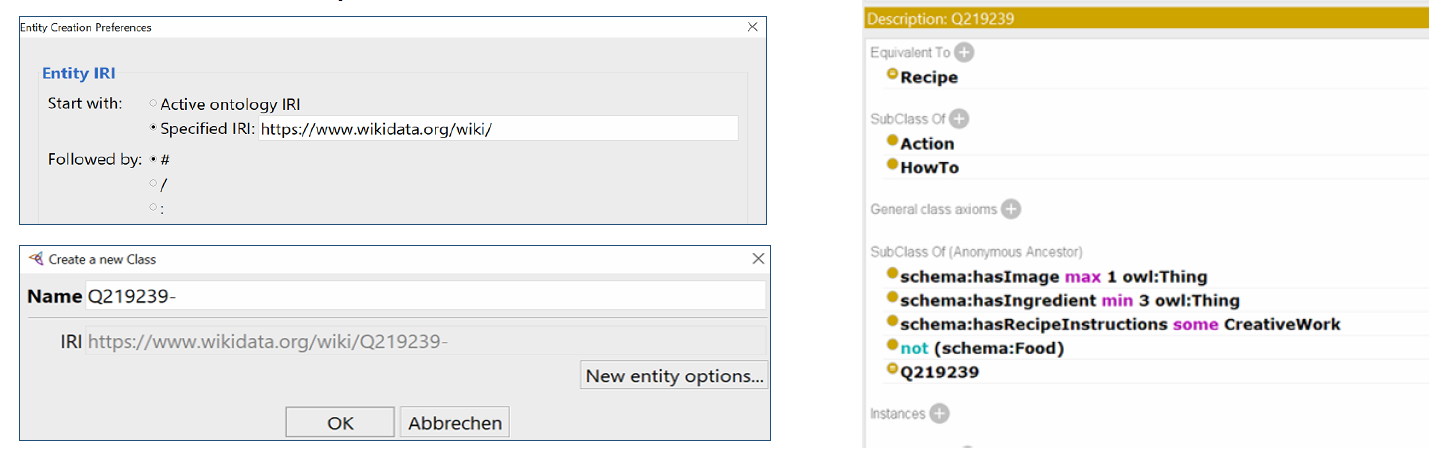
\includegraphics[width=15cm]{pictures/lod_linking.png}
  \caption{Create a link to Wikidata}
  \label{fig:lod}
\end{figure}
\noindent
\\ \\
First we create a new class in ``Protege'' while specifying the IRI in the preferences to link it to Wikidata. We name the entity we want to create the same as the Q-identifier from Wikidata (since it is the representation of the Wikidata entity). \\ \\
After that we now set the to classes in ``Protege'' as equal. As shown on the right side in Figure \ref{fig:lod} the subclasses are automatically inferred by the program. \\ \\
So after the linking is done we also started a reasoner to infer some extra constraints for the classes.\\ \\
Together with the OWL axioms (described in the next section) we exported and used the made changes to the ontology.

\subsection{OWL Axioms}
We used OWL axioms in our project to associate class and property IDs with complete specifications of their characteristics. We also used it to give other logical information about classes and properties. \\
Each class axiom in OWL contains a collection of more-general classes and a collection of local property restrictions in the form of restriction constructs. The restriction construct gives the local range of a property, how many values are permitted, and/or a collection of required values. The OWL axioms which we defined for our ontology can be seen in Figure \ref{fig:owl} and are directly saved in the ontology.

\begin{figure}[H]
  \centering
  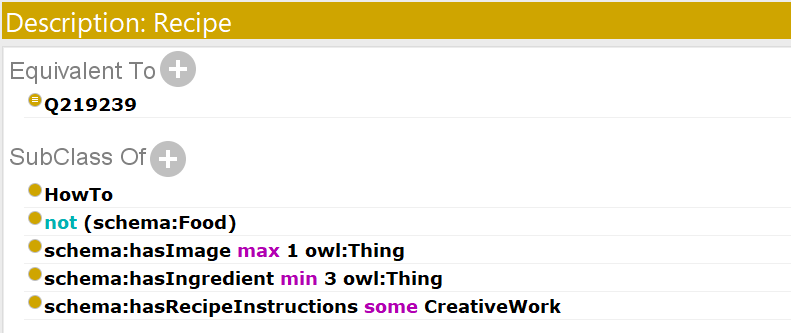
\includegraphics[width=12cm]{pictures/owl.png}
  \caption{OWL Axioms}
  \label{fig:owl}
\end{figure}
\noindent

\newpage

\section{Application}
\subsection{General Description}
In the following picture (Figure \ref{fig:front}) the main page for the user can be seen: \\

\begin{figure}[H]
  \centering
  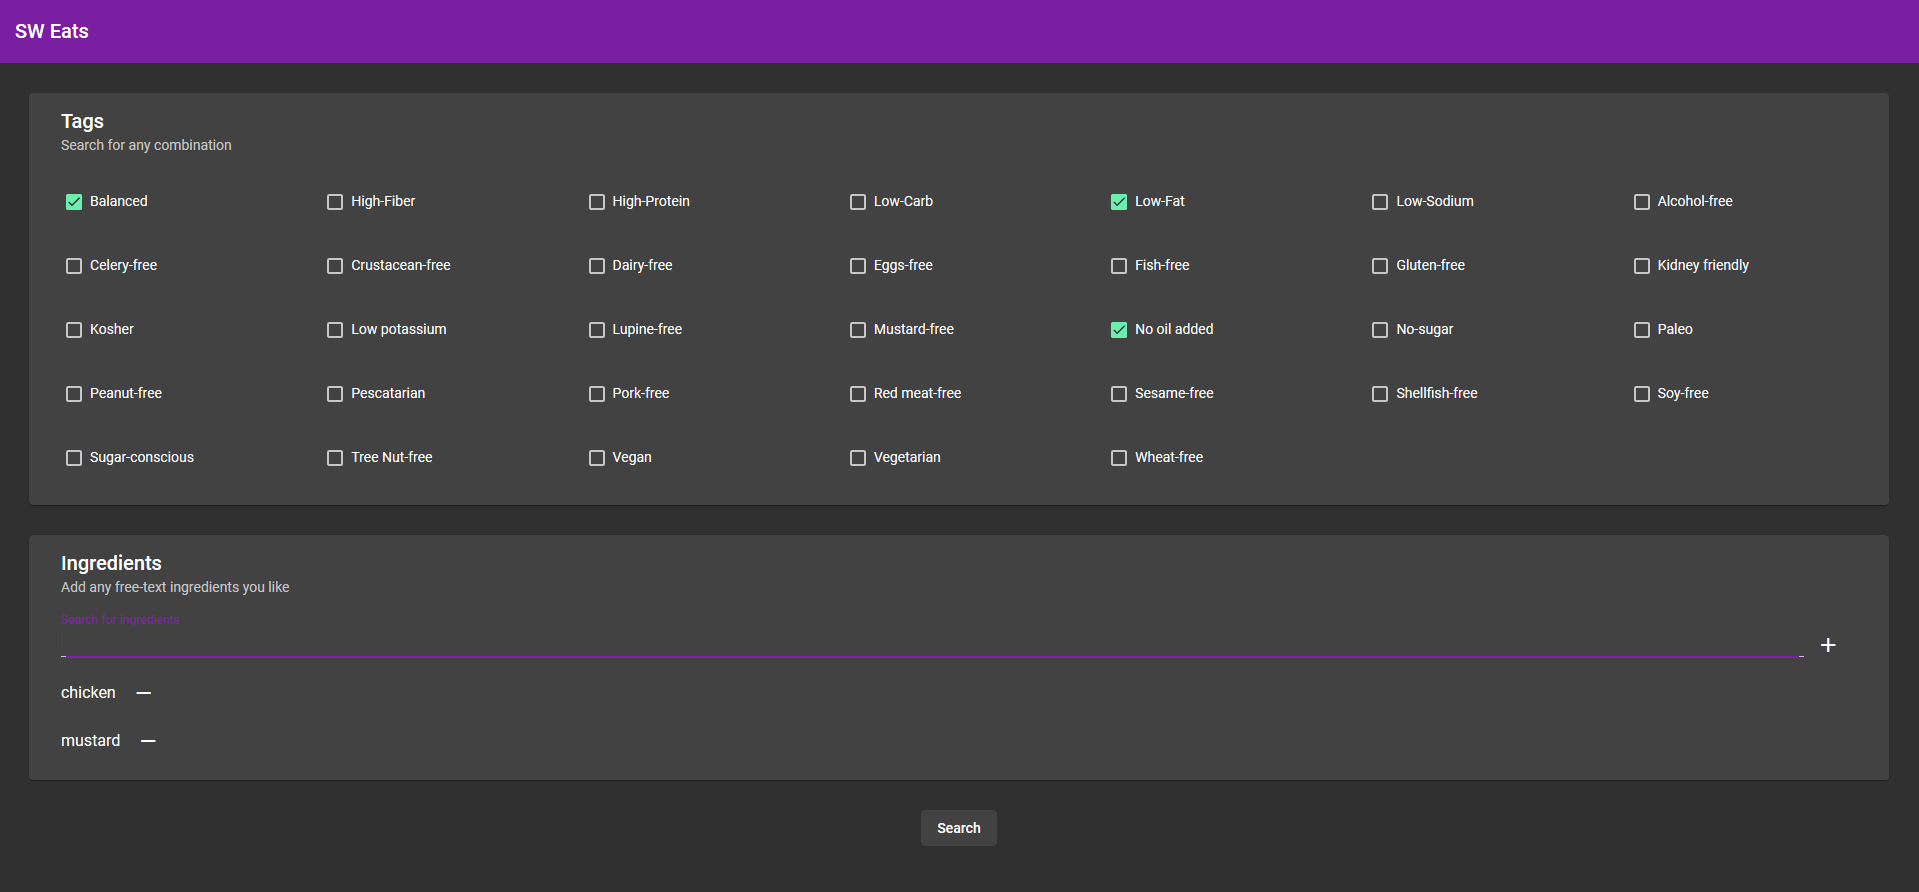
\includegraphics[width=15cm]{pictures/frontend.png}
  \caption{Main Page for our application}
  \label{fig:front}
\end{figure}
\noindent
\\ \\
Here the user can choose between different tags for the search which will be considered by our application. As already mentioned, we are using Edamam as our main data source and thus our tags shown in the picture follow directly the available tags (diet and health labels) stated by Edamam. The tags are set and unset by simple checkboxes. \\
In the other half of our starting page the input field for the ingredients can be found. Here the user can state single ingredients and add them to list of ingredients which is displayed directly below the input field. The user is also able to delete previously stated ingredients via the ``--'' button. \\ \\
Currently our database stores approximately 4500 different recipes which are considered when performing a search through our application.

\subsection{Architecture}
Basically our architecture consists of three main components shown in Figure \ref{fig:arch}:

\begin{figure}[H]
  \centering
  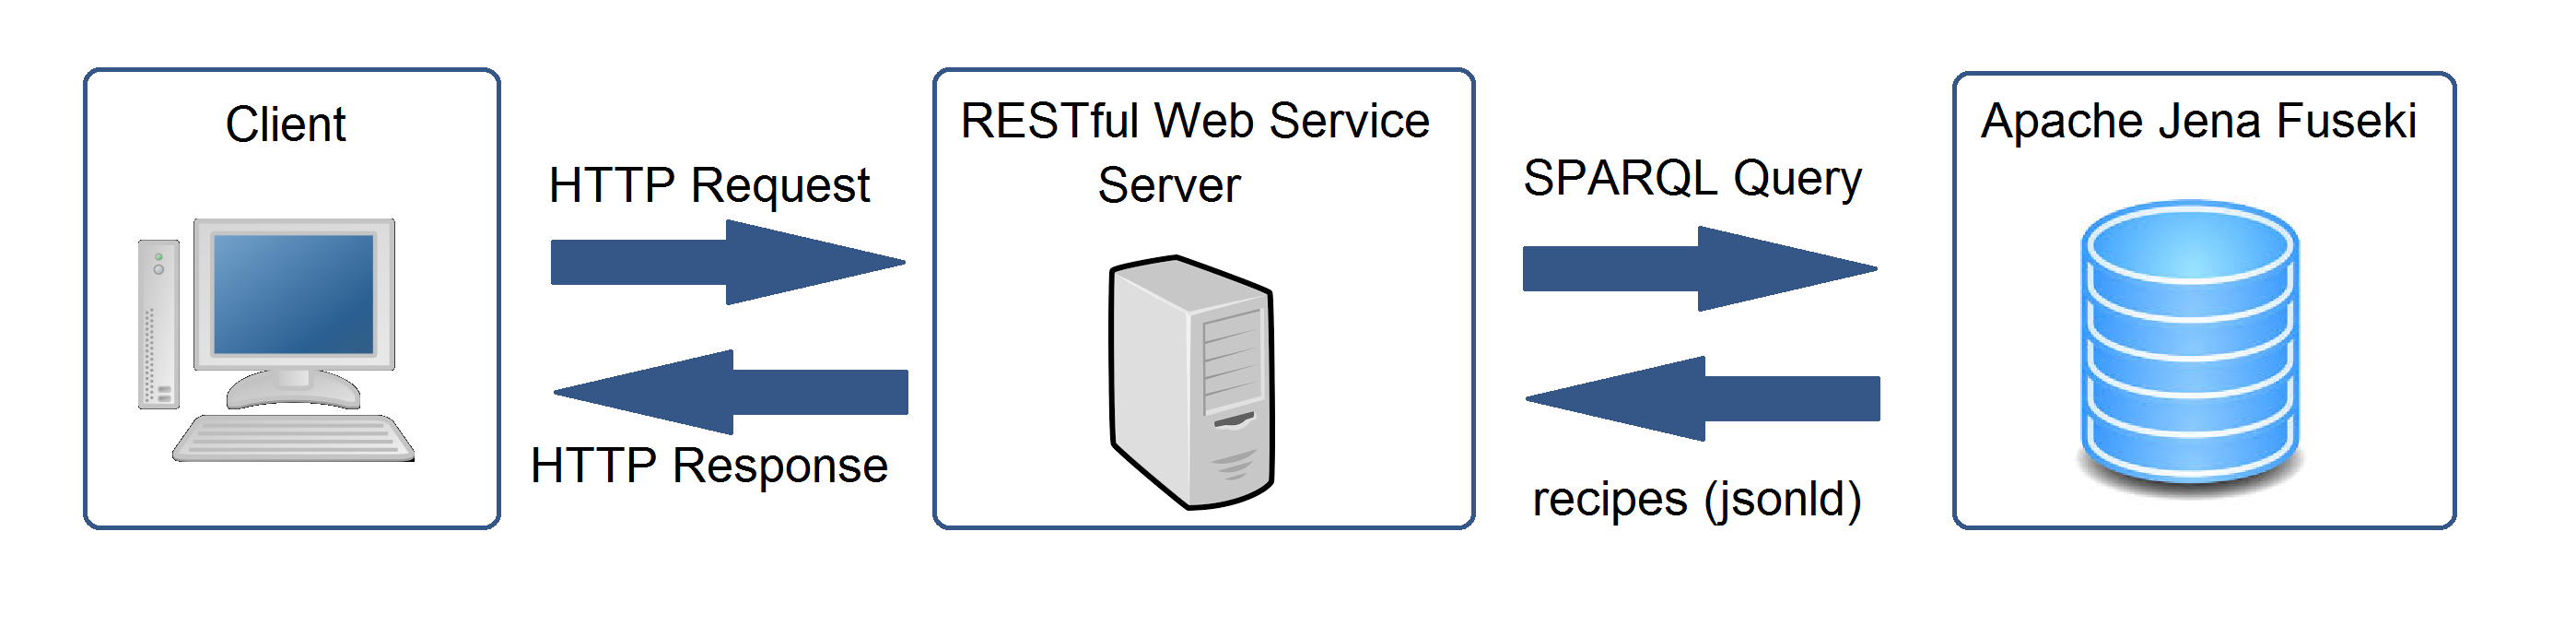
\includegraphics[width=12cm]{pictures/app.png}
  \caption{Basic architecture of our application}
  \label{fig:arch}
\end{figure}
\noindent
\\ \\
As seen in the picture the client (where the main page is displayed) sends a HTTP request with the desired tags and a list of the chosen ingredients to our RESTful Web Service Server. The RESTful Server parses the HTTP request (extracts the ingredients and tags from the HTTP request) and forms a dynamic SPARQL query, which is then sent to the Apache Jena Fuseki Server, where our triples are stored. The Fuseki Server then executes the query and responds with the desired data in Turtle-format (with the keyword DESCRIBE). We then take this result and parse it into jsonld which we hand back to the RESTful Web Service Server. This server forms a HTTP response with the results from the query and sends it back to the client where the results will be displayed properly.

\subsubsection{Client}
In this section we want to talk a little bit about the front-end of our application. The front-end is designed with ``Angular'' and is available on port 4200. Angular is a platform that makes it easy to build applications with the web. Angular combines declarative templates, dependency injection, end to end tooling, and integrated best practices to solve development challenges.  \\ \\
We performed an example request without any tags selected. The result is displayed in Figure \ref{fig:resp} to get an impression what our front-end looks like:

\begin{figure}[H]
  \centering
  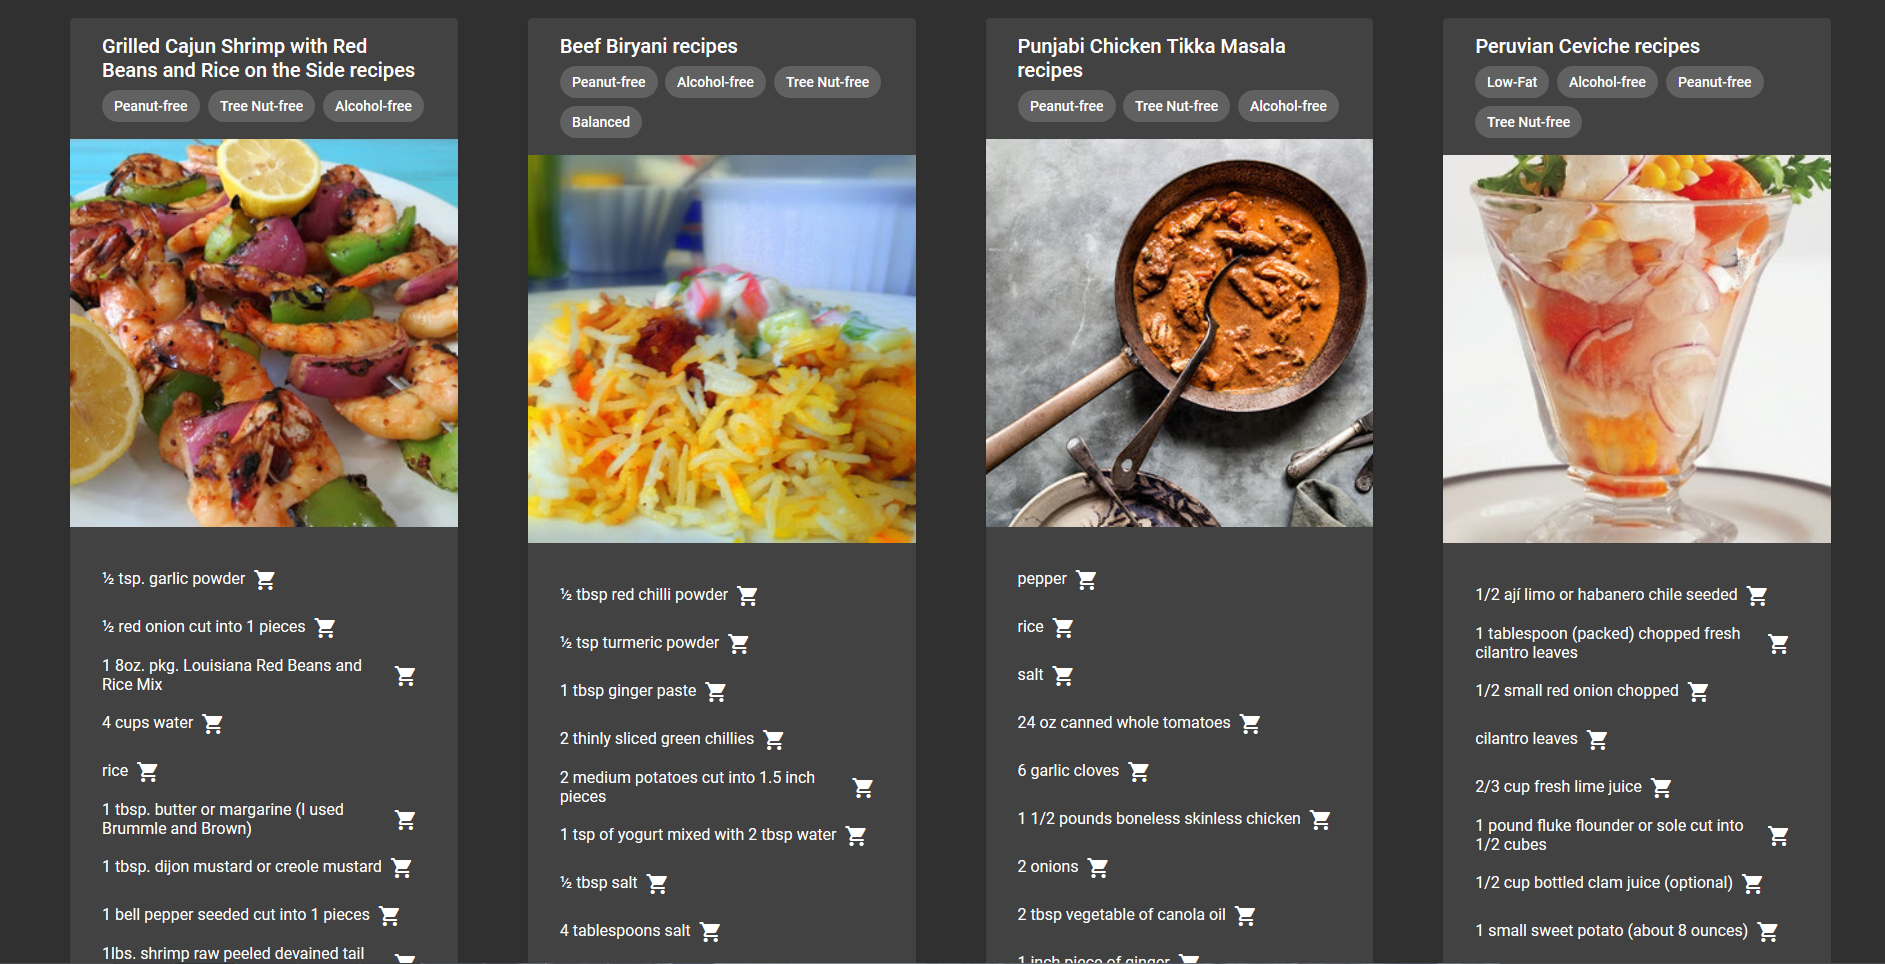
\includegraphics[width=14cm]{pictures/example_result.png}
  \caption{An example search}
  \label{fig:resp}
\end{figure}
\noindent
\\ \\
The user gets a nice looking result with the title of the recipe, the stored tags for each recipe, a picture which gives the user a first impression what the meal might look like after preparation and a list of ingredients. \\
Here we can also observe that directly after each listed ingredient there is a symbol to click on. When the user clicks on this symbol he is redirected to an online store which is called ``freshdirect'' where he or she can buy the corresponding ingredient. This is handled via a potentialAction (more specific: SearchAction).

\subsubsection{RESTful Web Service Server and Apache Jena Fuseki}
The backend part of our application starts with the RESTful Web Service Server which is available on port 8080. This server handles the HTTP request generated by the Client. It simply parses the desired ingredients and also the selected tags out of the HTTP request and hands it over to the second part of the backend, which is responsible for communicating with the Apache Jena Fuseki triple store. \\ \\
The second part of the backend gets the parsed input and forms a dynamic SPARQL query out of it. The generated Query is sent to the Apache Jena Fuseki Server which executes the query (Apache Jena Fuseki is located at port 3030). The result is then obtained and we parse it into a jsonld result which is then passed back to the front-end, where the results are displayed.\\

\paragraph{Levenshtein Filter}
We also implemented a Levenshtein Filter for the Fuseki Server so we can catch similar ingredients (e.g. it doesn't matter if an ingredient is written in lowercase or uppercase). This is implemented via the Levenshtein distance. This distance is a string metric for measuring the difference between two sequences or expressed more simple: the minimum single-character edits between to strings. So for the upper/lower case example the distance would be 1.

\paragraph{the dynamic SPARQL query}
The goal of this query is, to find entries in the triple store that match the requirements. These requirements are based on selected ingredients and tags. From these user-inputs a dynamic query is generated to get the desired schema:Recipe entries. The general idea is to find the matching subjects to a simple 'DESCRIBE' in the query is used to reconstruct the original recipe in its entirety. Since 'DESCRIBE' in Fusekis SPARQL yields a TTL-format a conversion to JSON-LD is essential since the results can be passed to any web-front-end without much modification of the data. An example application query (with ingredients: salt, butter, chicken and tag: Low-Carb) is shown in Figure \ref{fig:app_q}:

\begin{figure}[H]
  \centering
  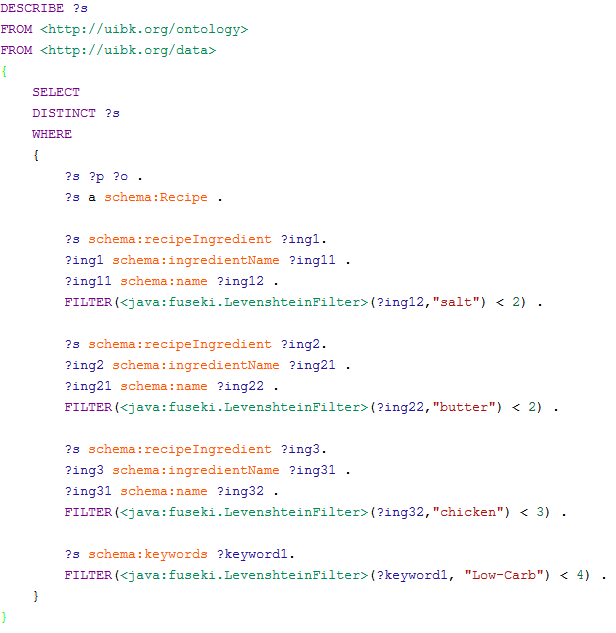
\includegraphics[width=12cm]{pictures/app_query.png}
  \caption{An example application query}
  \label{fig:app_q}
\end{figure}
\noindent
\\ \\
The first line is 'DESCRIBE ?s': This returns a TTL-Format RDF Graph reconstruction of a specified resource. In particular of the subject ?s which should ultimately be a schema:Recipe. The 'FROM' specifies the data and ontology graph. Now the ingredients need to be somehow looked up in the graph. First all possible values of '?s' must be a 'schema:Recipe'. Ingredients are linked to the recipe by the predicate 'schema:recipeIngredient'. This class has 3 classes in itself: 'schema:ingredientName', 'schema:ingredientAmount', 'schema:potentialAction'. Further the name of the ingredient can be found in the class 'schema:ingredientName'. Once the 'schema:ingredientName' object has been found a simple 'schema:name' will contain the actual name of an ingredient. The line 'FILTER(<java:fuseki.LevenshteinFilter$>$(?ing12,"salt") $<$ 2) .' applies a filter to match the ingredient name to a given search-word which is 'butter' in this case. Because user-error is sometimes inevitable the search-word is not directly matched to the entries. Instead a custom-made function 'LevenshteinFilter' extends the current SPARQL of the Fuseki to allow an error-margin when passing the search-words to the query. In this particular case any ingredient names will match satisfying the condition of 'LevenshteinFilter(ingredientNameIntripleStore,searchWord) $<$ 2'. The number '2' is automatically generated for the initial query and custom for every search-word and it simply depends on the length of the search-word. The same method is applied for other ingredients and tags.

\subsection{Data Crawling}
In this section we want to talk about our pipeline we implemented for data crawling. The pipeline itself is shown in Figure \ref{fig:pipe}:

\begin{figure}[H]
  \centering
  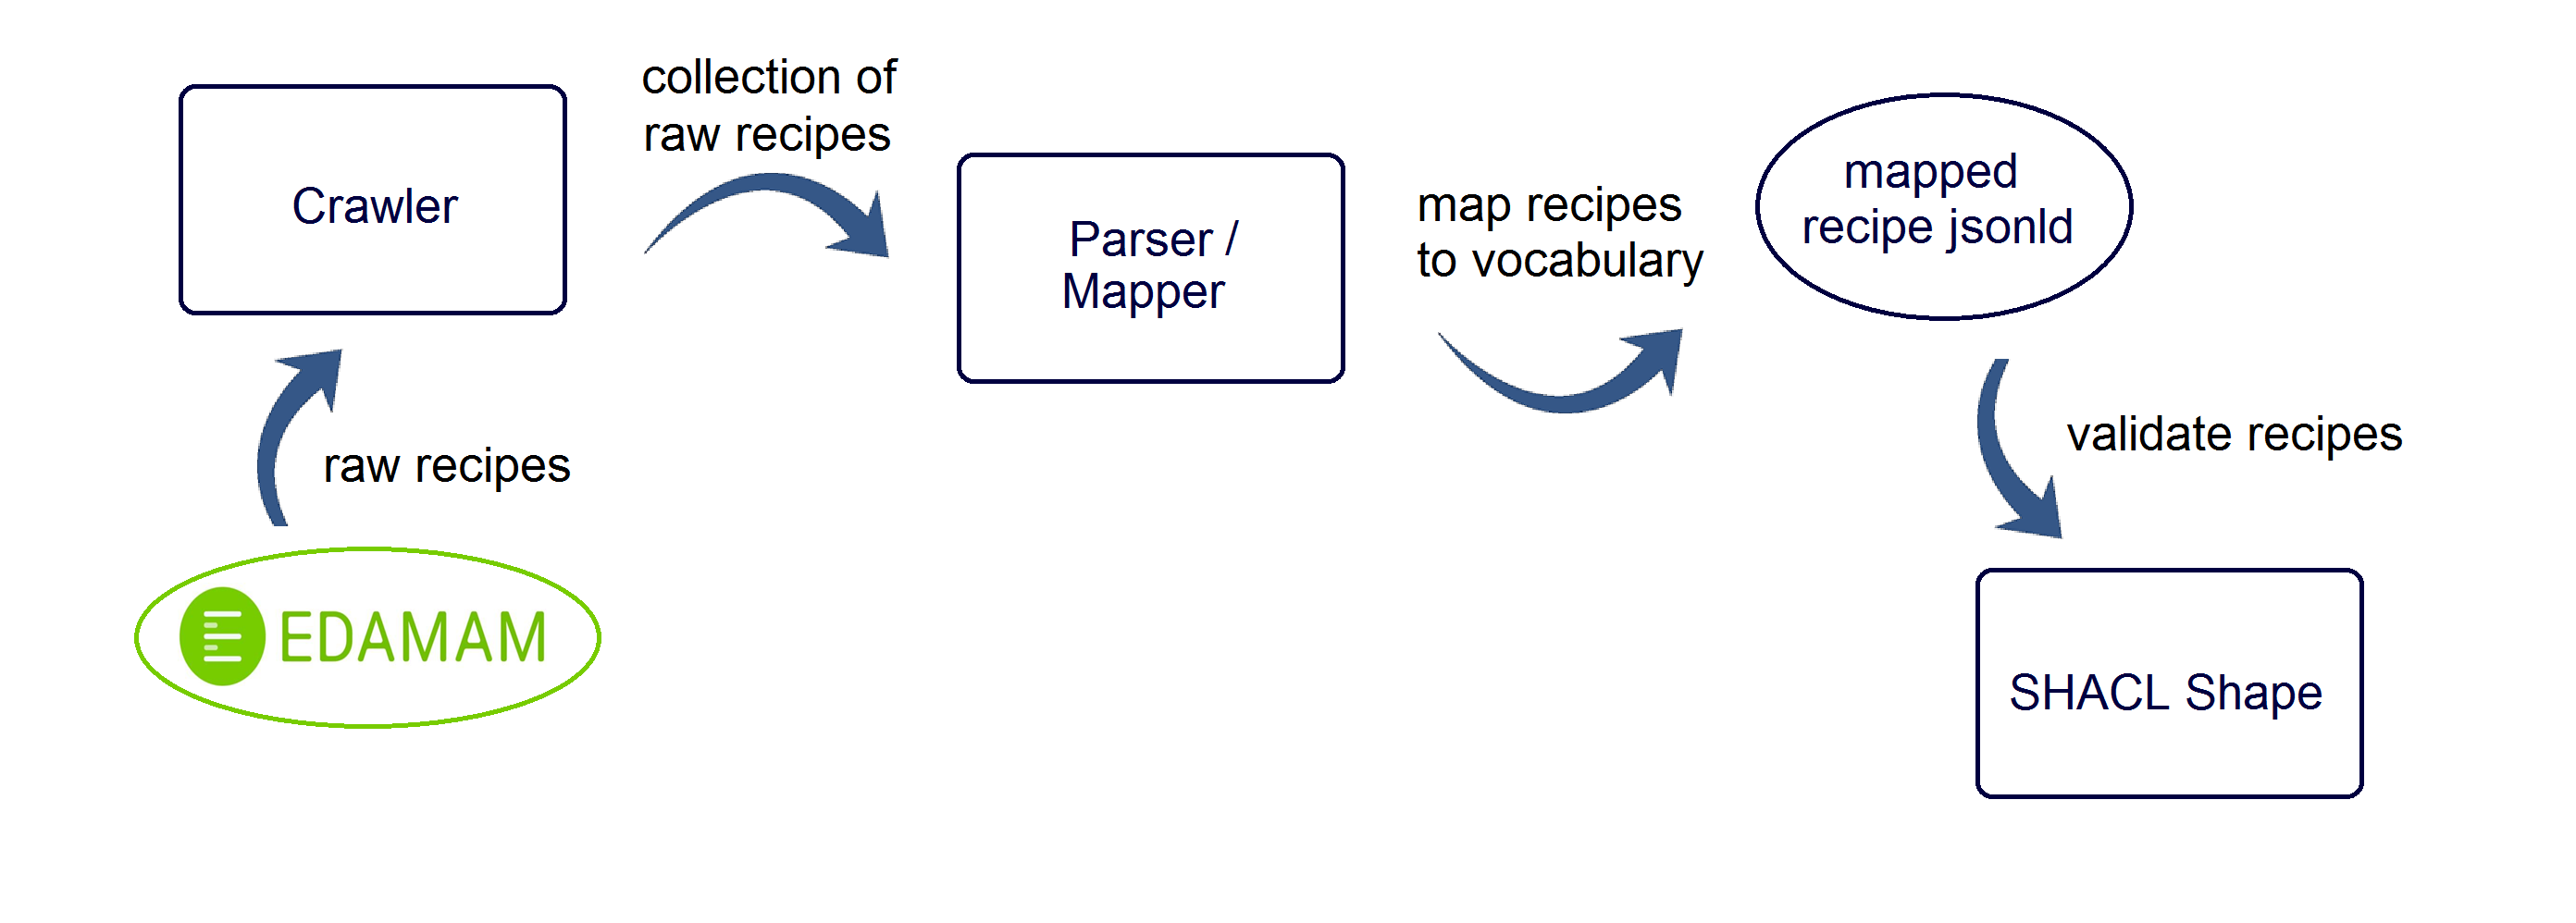
\includegraphics[width=12cm]{pictures/pipeline.png}
  \caption{The data crawling pipeline}
  \label{fig:pipe}
\end{figure}
\noindent
\\ \\
The pipeline startes with the main data source Edamam and our crawler. We basically state different cuisines as described before and the crawler goes through these categories and sends requests for each cuisine to the Edamam API. \\ \\
After we obtained the collection of the raw recipes we hand it over to the parser/mapper stage of our pipeline. In this stage we map our raw data to our vocabulary and form it into jsonld so we have a mapped-recipe-jsonld at the end of this stage. \\ \\
As the last stage of the pipeline we automatically validate our data with the SHACL shapes which are explained in the following section.

\subsection{SHACL Shapes}
As already mentioned in the first section we use SHACL shapes to validate our data. We do this to guarantee that only valid recipes are uploaded and stored into the Apache Jena Fuseki. Our SHACL shapes check whether the recipes have the correct format and furthermore if the individual properties have the correct data type. \\ \\
For this validation we have written a java program, which uses the shape and checks it against every recipe file. Any of the recipe files that cause a violation will be made invalid. After being made invalid our program deletes the incorrect recipe from the recipe file and makes the affected recipe file valid again. \\ \\
If a recipe file does not cause any violation it can safely be uploaded and stored into the Fuseki. The uploading process again is handled by a java program which automatically uploads all correct recipe files. A graphic representation of this process is shown in Figure \ref{fig:shacl}.

\begin{figure}[H]
  \centering
  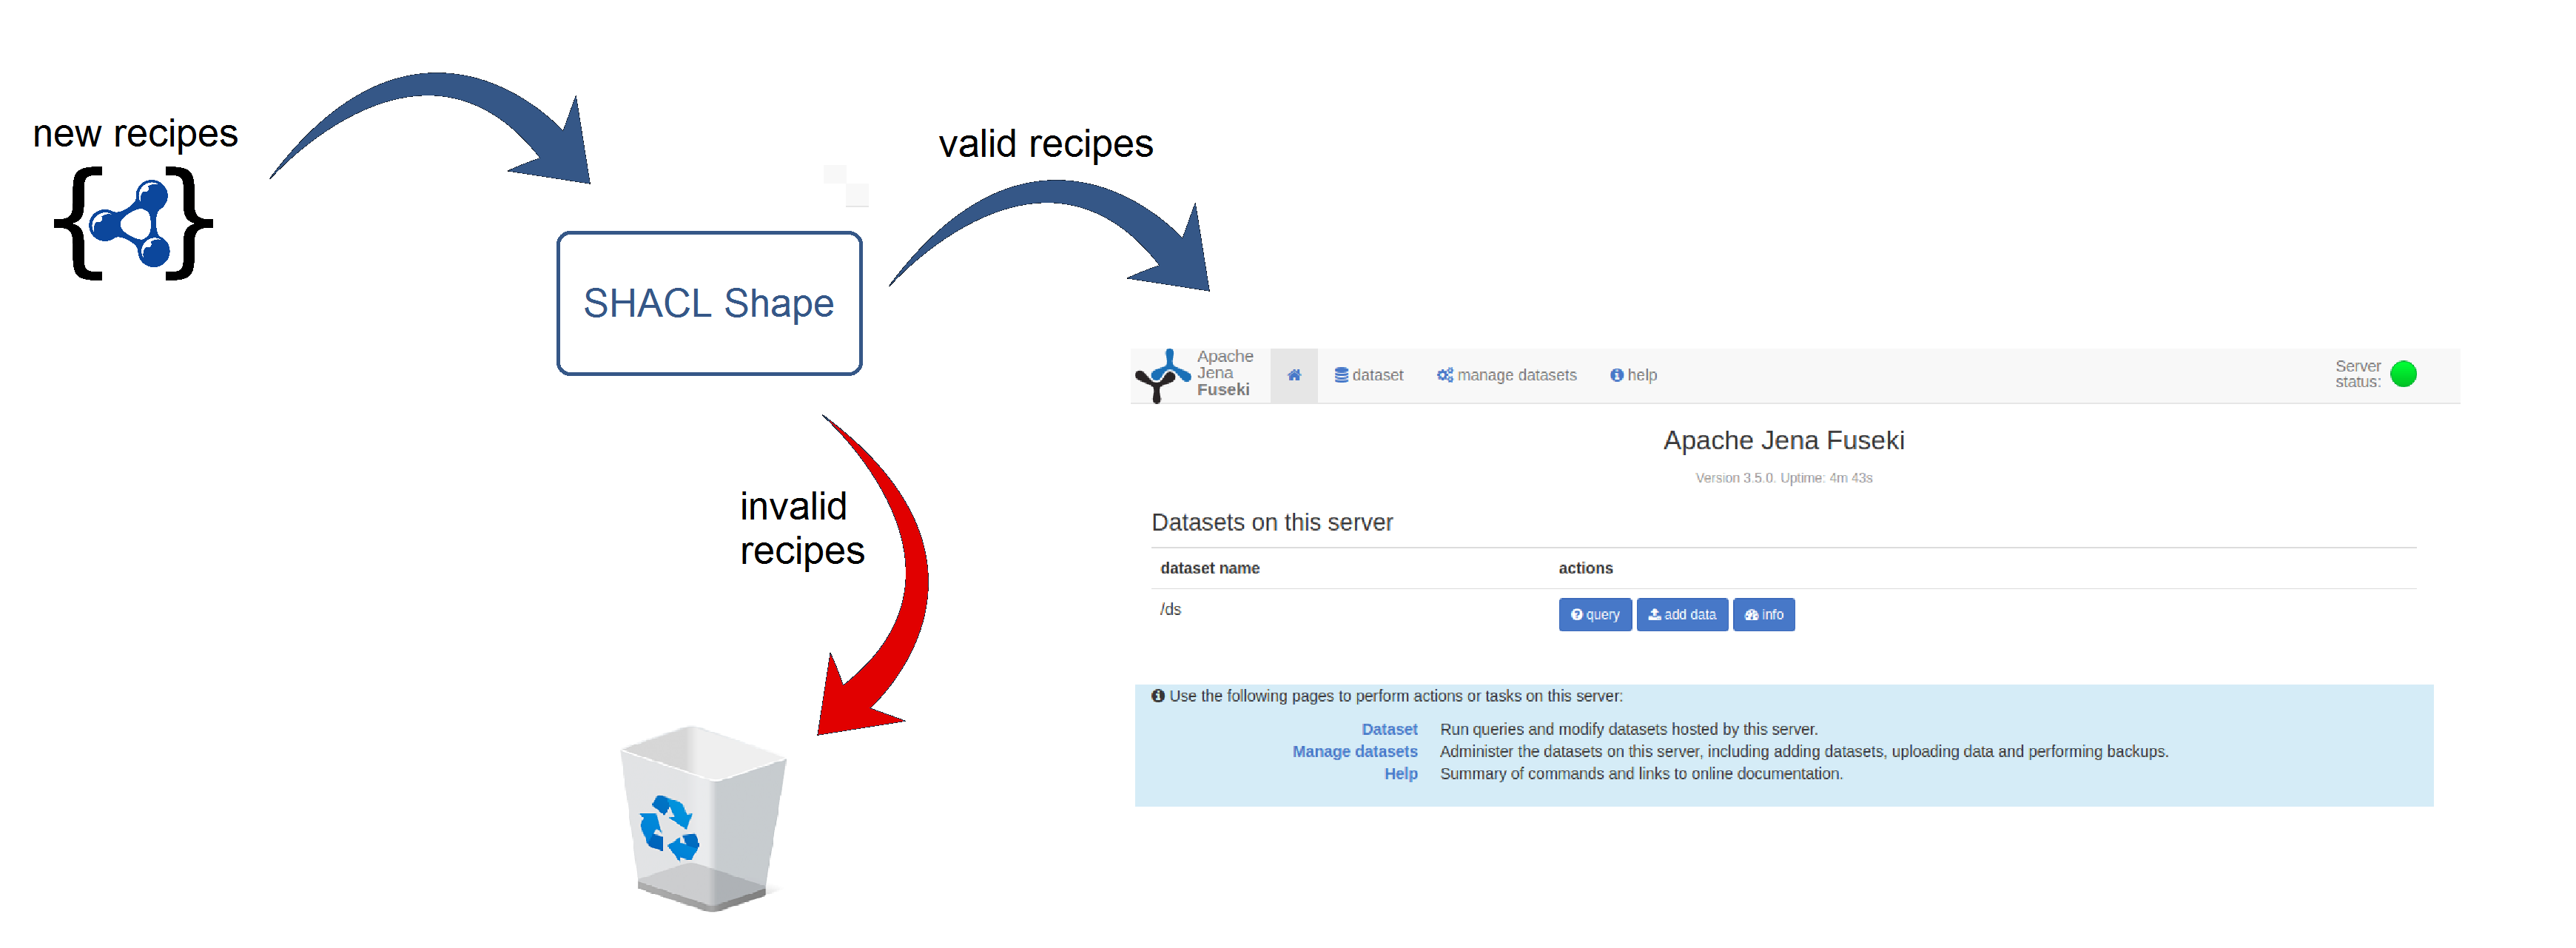
\includegraphics[width=12cm]{pictures/shacl.png}
  \caption{SHACL Representation}
  \label{fig:shacl}
\end{figure}
\noindent
	
\section{Conclusion}
The aspects of Semantic Web learned throughout the semester were all used in the project. Some of them are used in the application, while others are an important part of the data crawling process or the preparation of the data. All in all, the project was an interesting introduction to Semantic Web and taught us how to combine and leverage the different aspects of Semantic Web.
	

\end{document}	